%=============================================================================
\section{Introduction}
%=============================================================================

In the CCM Tools framework, a subset of OMG's Interface Definition Language
(IDL3) is used to define components, interfaces and parameters, as shown in 
Fig.~\ref{figure:IDLSubSet}.

\begin{figure}[htbp]
    \begin{center}
        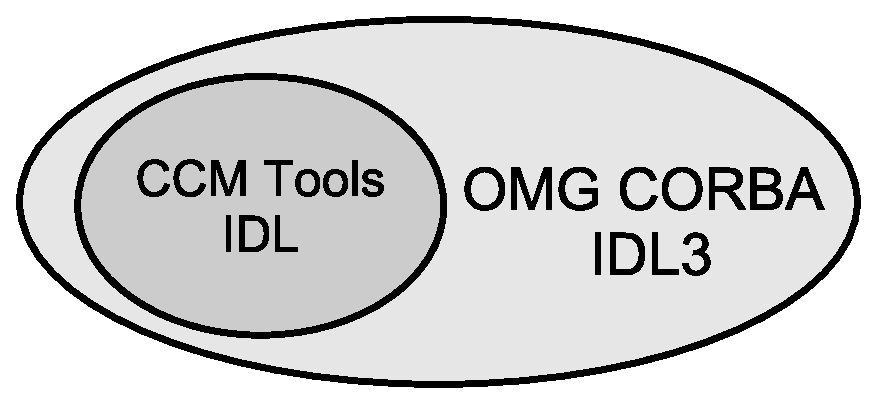
\includegraphics [width=10cm,angle=0] {figures/IDLSubSet}
        \caption{ CCM Tools support a subset of OMG's Interface Definition Language.}
        \label{figure:IDLSubSet}
    \end{center}
\end{figure}

Using an explicit IDL, we can define the structure of component--based
software systems completely independent of any particular programming 
language (e.g. C++ or Java).
Also, a clear separation between system design and implementation is 
guaranteed.

\newpage
